\documentclass[a4paper,12pt]{report}
\usepackage{hyperref}
\usepackage[table]{xcolor}
\usepackage{listings}
\usepackage{lmodern}
\usepackage[left=0.75in, right=0.75in, top=0.75in, bottom=0.75in]{geometry}
\usepackage{graphicx}
\usepackage{amsmath,amssymb}
\usepackage{tikz}
\usepackage{pgfplots}
\usepackage{subfigure}
\usepackage{enumerate}
\usepackage{tcolorbox}
\usepackage{fancyhdr}
\usepackage{setspace}
\usepackage{cancel}
\usepackage{placeins}
\usepackage{multirow}
\usepackage{algorithm2e}
\usepackage{booktabs}
\usepackage{bbding}
\pagecolor{white}
\color{black}

\pagestyle{fancy}

\hypersetup{%
  colorlinks=true,% hyperlinks will be black
  linkbordercolor=red,% hyperlink borders will be red
  pdfborderstyle={/S/U/W 1}% border style will be underline of width 1pt
}

\newcommand{\soln}{\\ \textbf{Solution}: }
\newcommand{\bkt}[1]{\left(#1\right)}

\lhead{MA5892: NMSC}
\chead{End Semester Exam}
\rhead{Roll number: PH15M015}

\begin{document}
\doublespacing
\begin{enumerate}

    \item An integral of the form $\displaystyle \int_{0}^{1} f(x) dx$ was computed
    by two students using trapezoidal rule with end point corrections involving only
    the first derivative. The first student reported the value as $0.8$ using a grid
    spacing of $h$, while the second student reported the value as $0.75$ using a grid
    spacing of $h/2$. A smart, lazy student from NMSC class enters their discussion
    and gives a better answer of the integral with a higher order of accuracy by processing
    the information above. How did he do it? What was his answer? What is the order of
    accuracy of his answer?

    \item Gaussian quadrature:
    \begin{itemize}
        \item Find the first three monic polynomials (i.e., till quadratic) on $[0, 1]$
        orthogonal with respect to the inner product

            \begin{equation*}
            \langle f, g \rangle = \int_{0}^{1} \frac{x}{\sqrt{1 - x^{2}}} f(x) g(x) dx
            \end{equation*}

        \item Use the above to find a quadrature formula of the form

            \begin{equation*}
            \int_{0}^{1} \frac{x}{\sqrt{1 - x^{2}}} f(x) dx = \sum_{i=0}^{n} a_{i} f(x_{i})
            \end{equation*}

        that is exact for all $f(x)$ of degree $3$.

        \item Use the above to evaluate $\displaystyle \int_{0}^{1} \frac{x \sin(x)}
        {\sqrt{1 - x^{2}}} dx$
    \end{itemize}

    \item Comment on using the Newton method to compute the root of the function $f(x)
    = x^{1/3}$, i.e., if your initial guess is $x_{0} = 1$, what would be the value of
    $x_{n}$? Does the method converge to the root we want?

    \item It is given that a sequence of Newton iterates converge to a root $r$ of the
    function $f(x)$. Further, it is given that the root $r$ is a root of multiplicity
    $2$, i.e., $f(x) = (x - r)^{2} g(x)$, where $g(r) \ne 0$. It is also given that the
    function $f$, its derivatives till the second order are continuous in the
    neighbourhood of the root $r$. If $e_{n}$ is the error of the $n^{th}$ iterate,
    i.e., $e_{n} = x_{n} - r$, then obtain

        \begin{equation*}
        \lim_{n \rightarrow \infty} \frac{e_{n+1}}{e_{n}}
        \end{equation*}

    \item \textbf{Bonus question:} What happens to the above if the root $r$ has a
    multiplicity $m$?

    \item Compute $\displaystyle \int_{-1}^{1} e^{-x^{2}} dx$ using the

    \begin{enumerate}
    \item Trapezoidal rule
    \item Trapezoidal rule with end corrections using the first derivative
    \item Trapezoidal rule with end corrections using the first derivative and third
    derivatives
    \item Gauss-Legendre quadrature
    \end{enumerate}

    \begin{itemize}
    \item Perform this by subdividing $[-1, 1]$ into $N \in \{2, 5, 10, 20, 50, 100\}$ 
    panels.
    \item Plot the decay of the absolute error using the above methods.
    \item You may obtain the exact value of the integral up to $20$ digits using
    wolfram alpha.
    \item Make sure the figure has a legend and the axes are clearly marked.
    \item Ensure that the font size for title, axes, legend are readable.
    \item Submit the plots obtained, entire code and the write-up.
    \end{itemize}
        
    \textbf{Program:}
    \lstinputlisting[language=Python]{Scripts/program6.py}

    \begin{figure}[ht!]
    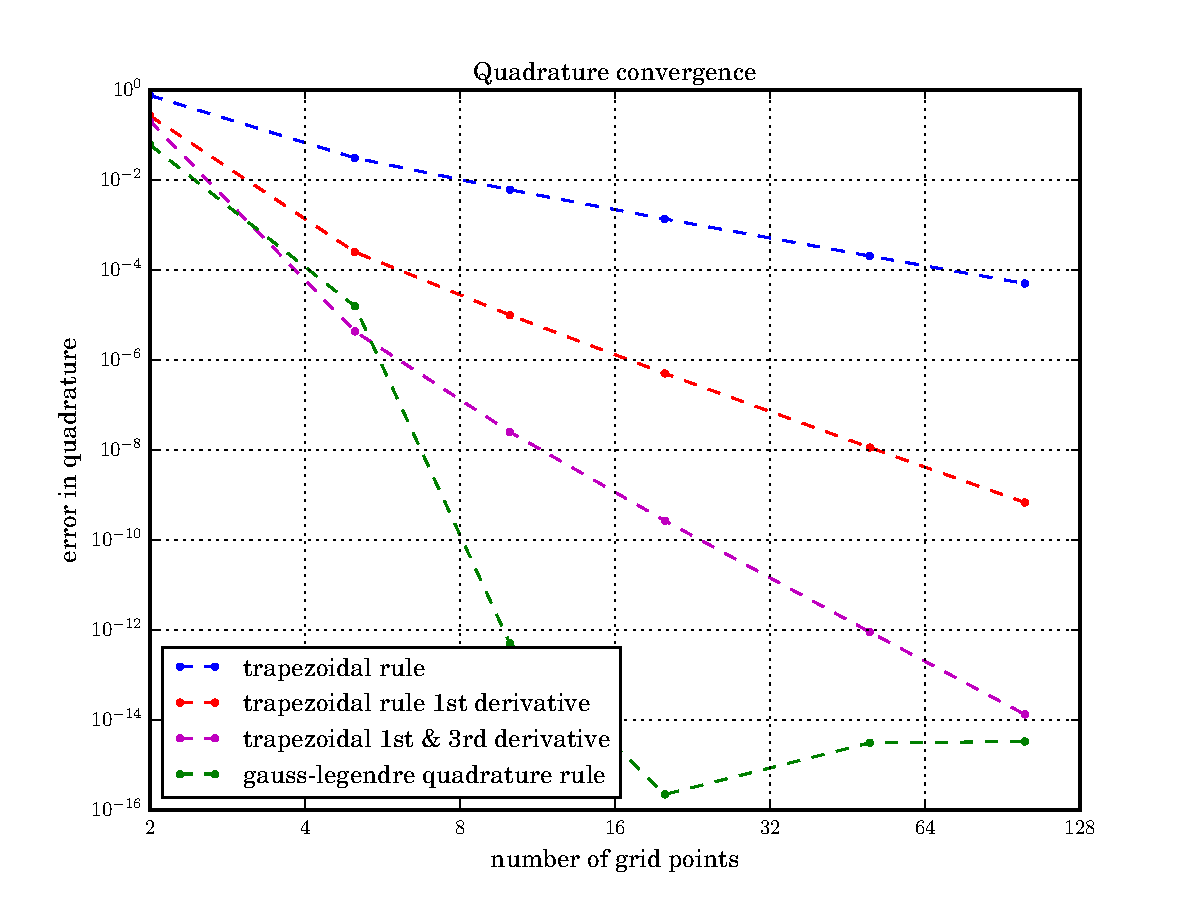
\includegraphics[width=0.9\linewidth]{Scripts/program6.pdf}
    \end{figure}

    \item Evaluate $I = \displaystyle \int_{0}^{1} \frac{e^{-x}}{\sqrt{x}} dx$ by
    subdividing the domain into $N \in \{5, 10, 20, 50, 100, 200, 500, 1000\}$ panels.

    \begin{enumerate}
    \item Using a rectangular rule
    \item Make a change of variables $x = t^{2}$ and use rectangular rule on new variable.
    \end{enumerate}

    \begin{itemize}
    \item Plot the decay of the absolute error using the above two methods.
    \item You may obtain the exact value of the integral up to $20$ digits using wolfram alpha
    \item Compare the two methods above in terms of accuracy and cost.
    \item Explain the difference in solution, if any.
    \item Make sure the figure has a legend and the axes are clearly marked.
    \item Ensure that the font size for title, axes, legend are readable.
    \item Submit the plots obtained, entire code and the write-up.
    \end{itemize}

    \textbf{Program:}
    \lstinputlisting[language=Python]{Scripts/program7.py}

    \begin{figure}[ht!]
    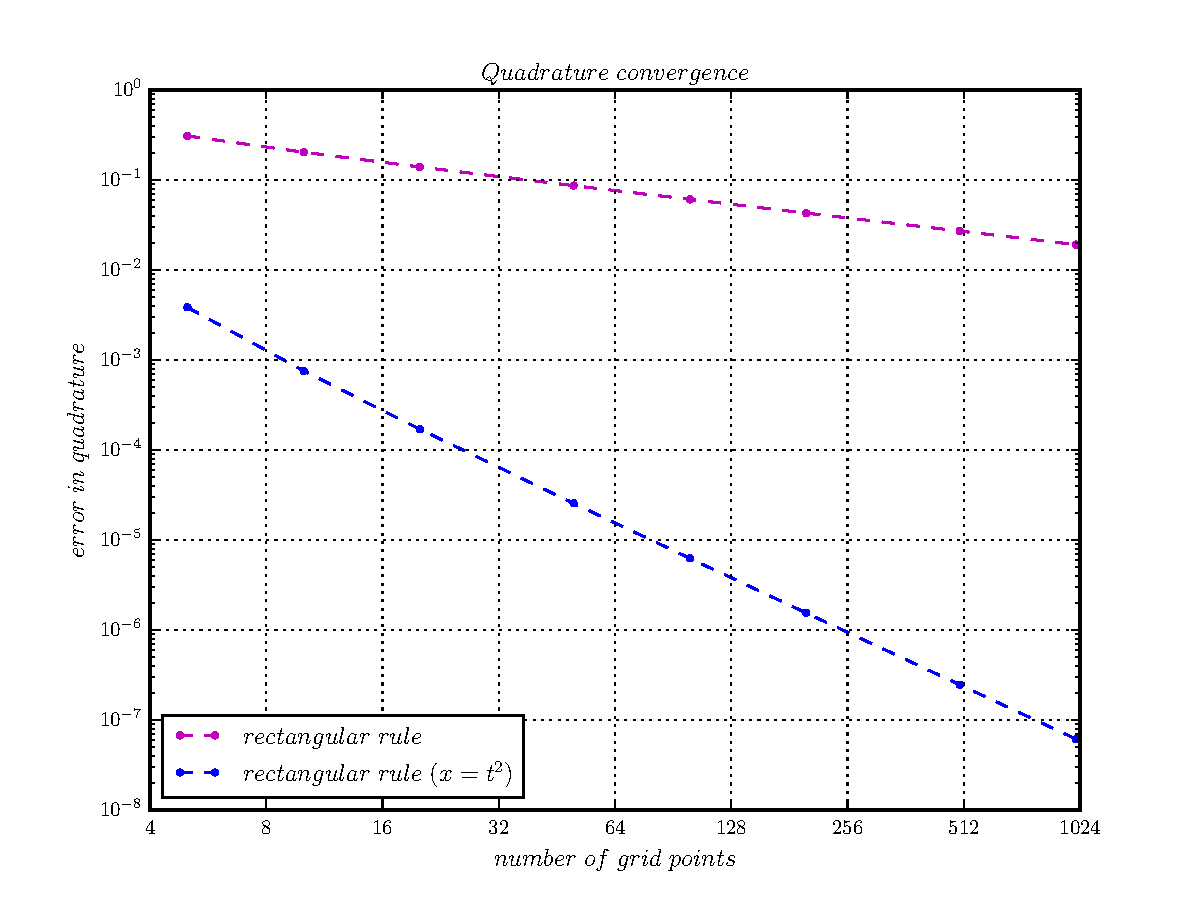
\includegraphics[width=0.9\linewidth]{Scripts/program7.pdf}
    \end{figure}

    \item Consider the motion of a simple pendulum. The restoring force is $mg \sin \theta$
    and hence the governing equation is

    \begin{equation*}
    mL \frac{d^{2} \theta}{dt^{2}} + mg \sin(\theta) = 0
    \end{equation*}

    Let the length of the string be $g$. Hence, the governing equation simplifies to
                    
    \begin{equation*}
    \frac{d^{2} \theta}{dt^{2}} + \sin(\theta) = 0
    \end{equation*}

    At the initial time, the pendulum is pulled to an angle of $\theta = 30^{\circ} =
    \displaystyle \frac{\pi}{6}$
    before being let loose without any velocity imparted. Write a code to solve for the
    motion of the pendulum till $t = 100$ seconds using

    \begin{enumerate}
    \item Forward Euler
    \item Backward Euler
    \item Trapezoidal Rule
    \end{enumerate}

    \begin{itemize}
    \item Recall that you need to reformulate the second order differential equation as a
    system of first order differential equation.
    \item Vary your time step $\Delta t$ in $\{0.01, 0.02, 0.05, 0.1, 0.2, 0.5, 1, 2, 5,
    10, 20\}$.
    \item For each $\Delta t$ plot the solution obtained by the three methods on a separate
    figure till the final time of $100$.
    \item Discuss the stability of the schemes. From your plots, at what $\Delta t$ do these
    schemes become unstable (if at all they become unstable)?
    \item Analyse the stability of the three numerical methods to solve the differential
    equation by approximating $\sin(\theta)$ to be $\theta$.
    \item Make sure each figure has a legend and the axes are clearly marked.
    \item Ensure that the font size for title, axes, legend are readable.
    \item Submit the plots obtained, entire code and the write-up.
    \end{itemize}

\end{enumerate}
\end{document}
